
\begin{enumerate}
    \item In figure 3.60, $0$ is the centre of a circle, AB is a chord and AT is the tangent at A. If $\angle AOB = 100^\circ$, then $\angle BAT$ is equal to
    \begin{figure}[h]
        \centering
        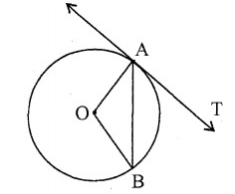
\includegraphics{figs/circfig_1.jpg}
        \caption{}
    \end{figure}    
    \begin{enumerate}
        \item $100^\circ$
        \item $40^\circ$
        \item $50^\circ$
        \item $90^\circ$
    \end{enumerate}\newpage
    \item In figure 3.61, PA and PB are tangents to the circle with centre O. If $\angle APB=100^\circ$, then $\angle OAB$ is
    \begin{figure}[h]
        \centering
        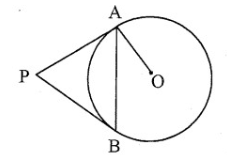
\includegraphics{figs/circfig_2.jpg}
        \caption{}
    \end{figure}
    \begin{enumerate}
        \item $30^\circ$
        \item $60^\circ$
        \item $90^\circ$
        \item $15^\circ$
  \end{enumerate}
    \item The radii of two circles are 4cm and 3cm respectively. The diameter of the circle having area equal to the sum of the area of the two circles (in cm) is
    \begin{enumerate}
        \item 5
        \item 7 
        \item 10
        \item 14
    \end{enumerate}
    \item 	Two concentric circles are of radii $7$ cm and $r$ cm respectively, where $r>7$. A chord of the larger circle, of length $48$ cm, touches the smaller circle. Find the value of $r$.
    \item In figure 3.62, APB and CQD are semi-circles of diameter 7 cm each, while ARC and BSD are semi-circles of diameter 14 cm each. Find the perimeter of the shaded region.[Use $\pi=\dfrac{22}{7}$]
    \begin{figure}[h]
        \centering
        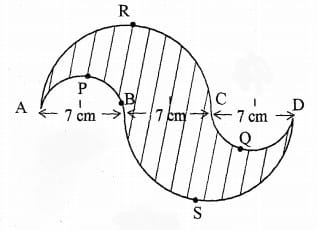
\includegraphics[width=5cm]{figs/circfig_3.jpg}
        \caption{}
    \end{figure}
    \item In figure 3.63, a triangle ABC is drawn to circumscribe a circle of radius 2cm such that the segments BD and DC into which BC is divided by the point of contact D are of lengths 4cm and 3cm respectively. If area of $\triangle ABC=21cm^2$, then find the lengths of sides AB and AC.
    \begin{figure}[h]
        \centering
        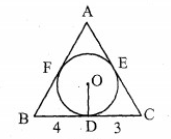
\includegraphics[width=4cm]{figs/circfig_4.jpg}
        \caption{}
    \end{figure}\\
    \item Find the area of the major segment $APB$, in figure 3.64, of a circle of radius $35cm$ and $\angle AOB=90^\circ$.[Use $\pi=\dfrac{22}{7}$]
     \begin{figure}[H]
        \centering
        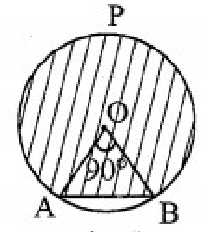
\includegraphics[width=5cm]{figs/circfig_5.jpg}
        \caption{}
    \end{figure}
    
    \item The radii of the circular ends of a bucket of height $15$ $cm$ are $14$ $cm$ and r $cm$ ($r<14$ $cm$). If the volume of bucket is $5390$ $cm^3$, then find the value of $r$.[Use $\pi=\dfrac{22}{7}$]

